%matplotlib inline: esto es para que las graficas aparescan a dentro.

\documentclass{article}
%Reporte de computacional
%matplotlib inline: esto es para que las graficas aparescan a dentro.
\usepackage{hyperref}
\usepackage{amsmath}
\usepackage{amsthm}
\usepackage{amssymb}
\usepackage{graphicx}
\usepackage{ifxetex}
\ifxetex
\usepackage{fontspec}
\else
\usepackage[T1]{fontenc}
\usepackage[utf8]{inputec}
\usepackage{lmodern}
\fi



\begin{document}
\title{Oscilador de Van de Pol}
\author{Ramses Pacheco Ortiz}
\date{14 de Abril Del 2018}
\maketitle  


\section{Introducción}
Esta práctica representa la actividad 8 del curso,la cual trabajamos con el modelo de Van der Pol prosiguiendo un poco con el tema de oscilaciones no conservativas mas adelante explicaremos mas a profundidad este modelo.

\vspace{0.1cm}
Para realizar esta actividad utilizamos la misma herramienta de python(jupyter lab) de las actividades 6 y 7 ,usando algunas bibliotecas de las actividades pasadas como Numpy,Matplotlib,Pylab y en particular odeint de scipy utilizado en actividades anteriores para realizar las integraciones.


\section{Modelo de Van der Pol}

El modelo de van der pol es un oscilador no conservativo con un amortiguamiento,su comportamiento esta dado por la siguiente expresion matematica:

\begin{center}
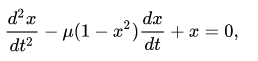
\includegraphics[height=1cm]{fig1.png}
\end{center}

En esta expresion $x$ es la posicion que esta en funcion del tiempo $t$  y $u$ es una constante que indica la no linealidad y la fuerza del amortiguamiento.

\subsection{Historia}

El oscilador de van der Pol fue descrito por el ingeniero y físico Balthasar van der Pol mientras trabajaba en Philips. Van der Pol encontró oscilaciones estables, que llamó oscilaciones de relajación,conocidas en la actualidad como ciclos límite, en circuitos que usaban válvulas de vacío. 

\vspace{0.1cm}

Van der Pol y su colega, van der Mark, informaron en septiembre de 1927 de Nature,que para determinadas frecuencias aparecía un ruido irregular, siempre cerca de las frecuencias de acoplamiento. Fue uno de los primeros descubrimientos experimentales de la Teoría del caos.

\vspace{0.1cm}

La ecuación de van der Pol tiene una larga historia en física y biología. Por ejemplo, en biología, Fitzhugh y Nagumo aplicaron la ecuación a un campo bidimensional en el modelo de FitzHugh-Nagumo para describir el potencial de acción de las neuronas. También se ha usado en sismología para modelar el comportamiento de dos placas en una falla.


\subsection{Forma Bidimensional}

El teorema de Liénard prueba que el sistema tiene un ciclo límite. Aplicando la transformación de Liénard:

\begin{center}
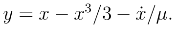
\includegraphics[height=1cm]{fig2.png}
\end{center}

donde el '.' indica derivada, la ecuación se puede escribir en forma bidimensional:

\begin{center}
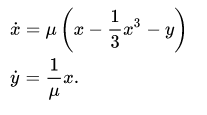
\includegraphics[height=3cm]{fig3.png}
\end{center}


\subsection{Resultados del oscilador no forzado}

Hay dos regímenes de funcionamiento interesantes para el oscilador no forzado:

\begin{itemize}
\item Cuando μ = 0, no hay amortiguamiento, y la ecuación queda:


\begin{center}
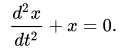
\includegraphics[height=1cm]{fig4.png}
\end{center}


\item

Cuando μ > 0, el sistema alcanzará un ciclo límite, en el que se conservará la energía. Cerca del origen $x = dx/dt = 0$ el sistema es inestable, y lejos del origen hay amortiguamiento.

\end{itemize}

\subsection{El oscilador de van der Pol forzado}

Utilizando una fuente de excitación sinusoidal Asin(ωt) la ecuación diferencial queda:

\begin{center}
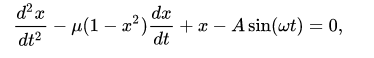
\includegraphics[height=1cm]{fig5.png}
\end{center}

en la que A es la amplitud de la ecuación de onda y ω su velocidad angular.


\subsection{Hamiltoniano para el oscilador de van der pol}

Tambien se puede escribir el hamiltoniano del oscilador del van der pol independiente del tiempo aumentando el sistema de unos de cuatro dimensiones, para esto primero tenemos que escribir el sistema por medio de ecuaciones diferenciales no lineales como las siguientes:

\begin{center}
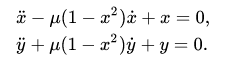
\includegraphics[height=1cm]{fig6.png}
\end{center}

De las cuales podemos obtener el hamiltoniano de la siguiente manera:


\begin{center}
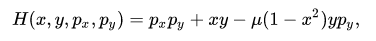
\includegraphics[height=1cm]{fig7.png}
\end{center}


donde $px$ y $py$son los momentos respectivos a $x$ y a $y$


\subsection{Circuitos electricos}

En 1920 van der pol constuyo el oscilador con un triodo o tetrodo. despues de que Reona Esaki el tunes del diodo en 1957,haciendo que el oscilador de van der pol con el circuito eléctrico fuera mas sencillo.

La expresión matematica del circuito esta dada por la siguiente ecuación:

\begin{center}
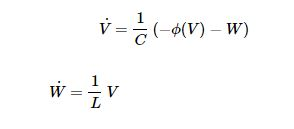
\includegraphics[height=2cm]{fig10.png}
\end{center}

La cual a su vez puede ser escrita como:

\begin{center}
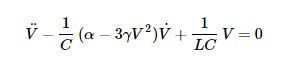
\includegraphics[height=2cm]{fig11.png}
\end{center}

\section{Exploracion de las soluciones del modelo en el Espacio Fase}

para realizar esta parte,cmabiaremos las condiciones iniciales, y se mantendra constante la mu=3.0,para llevar a cabo las siguientes graficas que mostraremos nos basamos en el codigo de la actividad anterio.

Cambiamos las condiciones iniciales para comprobar que verdaderamente convergia a la misma figura sin importar las condiciones iniciales.

A continuación mostraremos las graficas que se llevaron a cabo:

\begin{center}
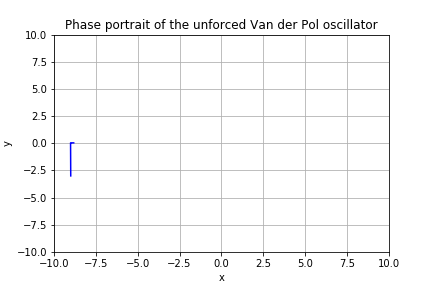
\includegraphics[height=5cm]{extra1_1.png}
\end{center}

\begin{center}
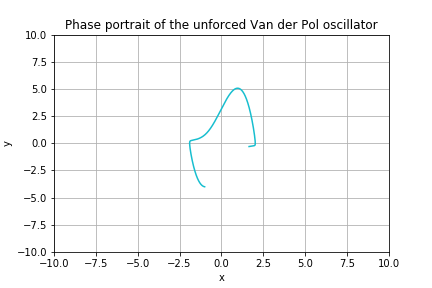
\includegraphics[height=5cm]{extra2.png}
\end{center}

\begin{center}
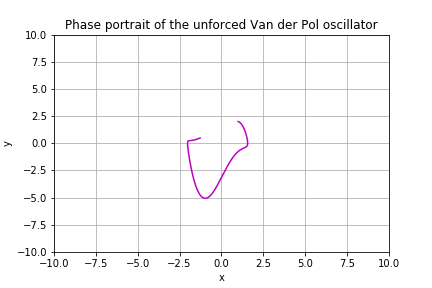
\includegraphics[height=5cm]{extra3.png}
\end{center}

\begin{center}
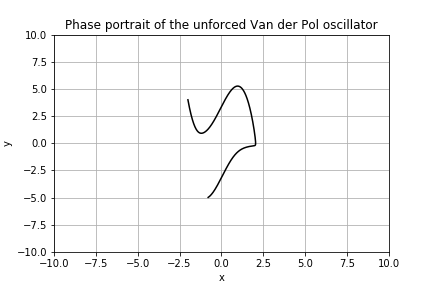
\includegraphics[height=5cm]{extra4.png}
\end{center}


\begin{center}
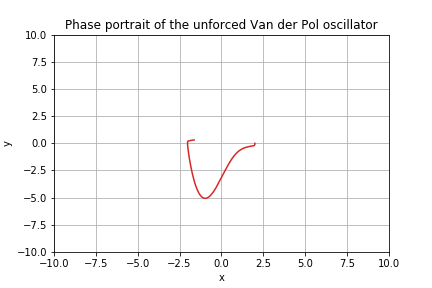
\includegraphics[height=5cm]{extra5.png}
\end{center}


como se puede observar sin inportar las condiciones que le pusimos siempre converge a la misma figura


\section{Resultados y Discusión}

En esta actividad realizamos 4 graficas basandonos en archivo de texto de wikipedia del oscilador van der pol

A continuacion se mostrara el codigo que se utilizo para realizar las graficas:

\begin{itemize}
\item Primera grafica


\begin{center}
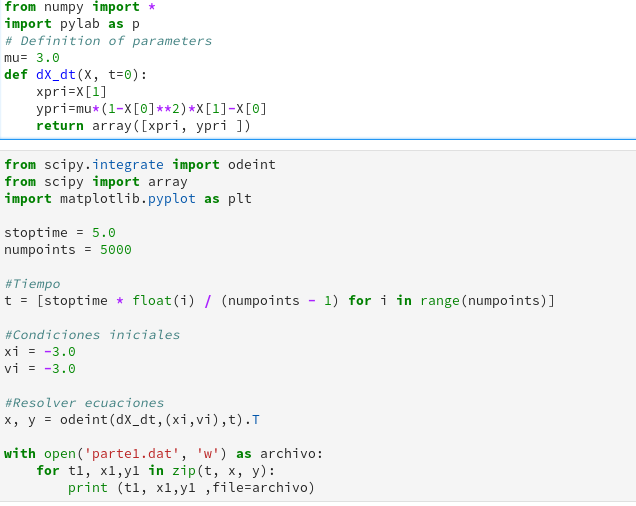
\includegraphics[height=6cm]{cod1.png}
\end{center}

En la imagen anterio se hixo los mismo pero cambiando las condiciones iniciales(x1,y2) y el nombre del archivo hasta realizar 5 partes, al final
 graficas estas cinco partes para juntarlas en una sola:
 
 
\begin{center}
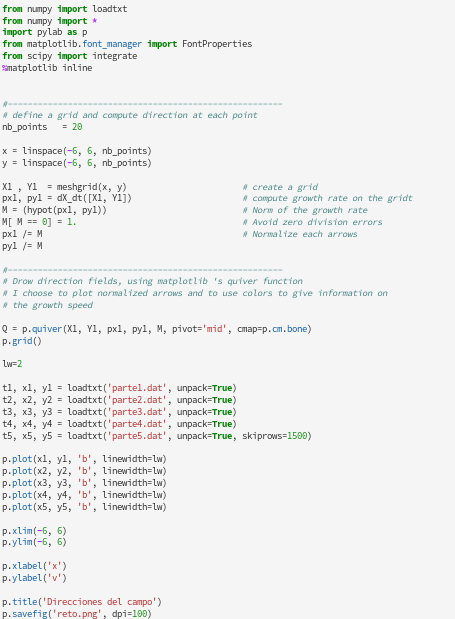
\includegraphics[height=12cm]{cod2.png}
\end{center}

A continuacion se mostrara la grafica resultante:

\begin{center}
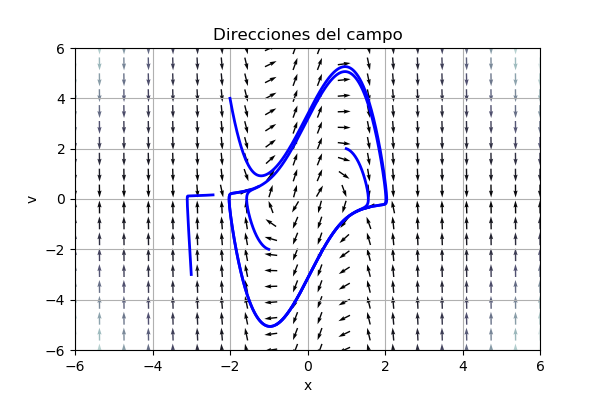
\includegraphics[height=6cm]{reto.png}
\end{center}




\item Segunda grafica

primeramente se definiola funcion van el por,despues en el codigo que se mostrara a continuacion muestra muchas varaibles debido a que son varias las condiciones iniciales
 
 \begin{center}
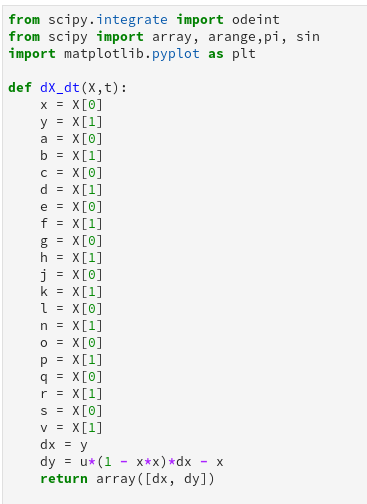
\includegraphics[height=8cm]{cod3.png}
\end{center}
 
A continuacion se mostrara la grafica:


 \begin{center}
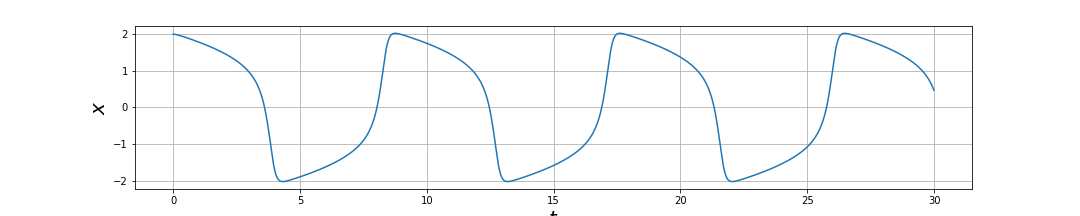
\includegraphics[height=3cm]{2dafig.png}
\end{center}


\item Tercera grafica

Para realizar la siguiente grafica se utilizo elsigueinte codigo:

\begin{center}
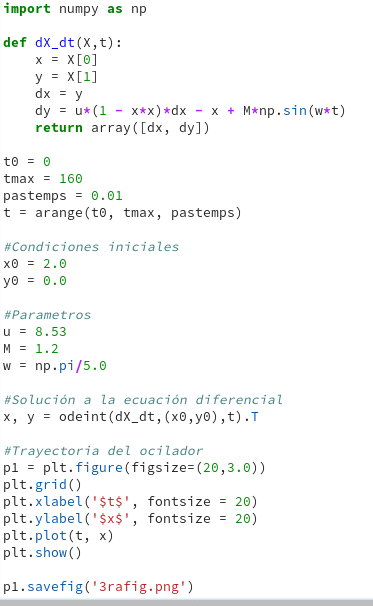
\includegraphics[height=10cm]{cod4.png}
\end{center}

La grafica resultante es:

 \begin{center}
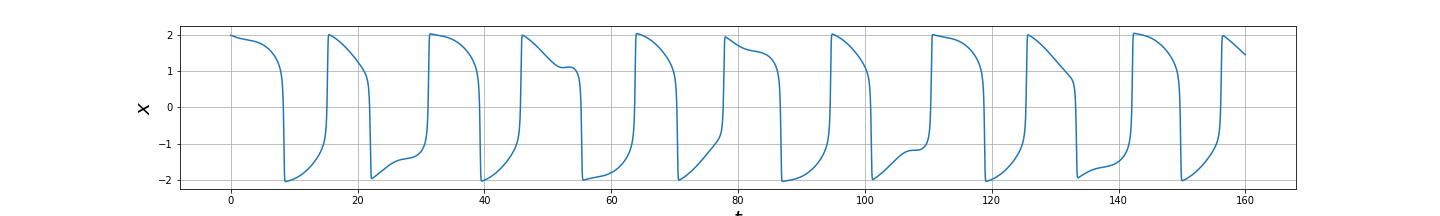
\includegraphics[height=3cm]{3rafig.png}
\end{center}




\item Cuarta y ultima grafica

Primero tubimos que juntar cada solucion de la ecuacion diferencial y despues graficamos las trayectorias de fase


\begin{center}
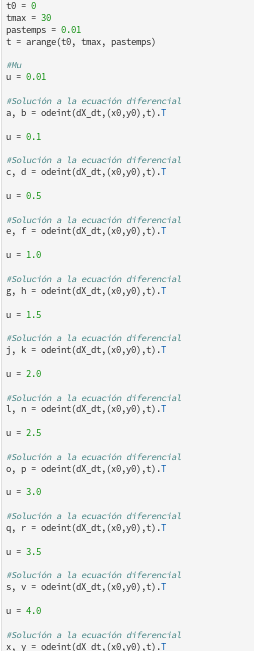
\includegraphics[height=10cm]{cod5.png}
\end{center}

\begin{center}
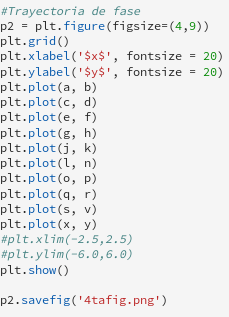
\includegraphics[height=6cm]{cod6.png}
\end{center}


A continuacion se mostrara la figura resultante:


\begin{center}
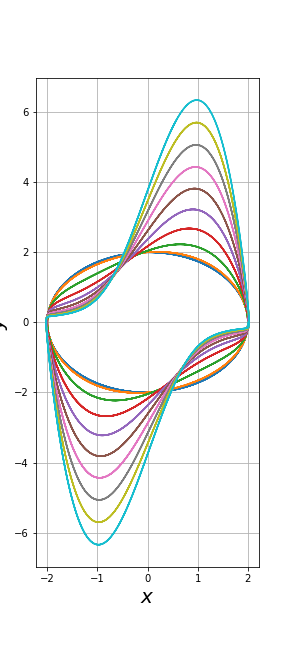
\includegraphics[height=6cm]{4tafig.png}
\end{center}

\end{itemize}


\section{Conclusiones}

Continuando con el tema de ecuacions diferanciales no lineales y comparando esta actividad con la anterior me paracio mas interesanta el sistema que trabajamos y respeto a las graficas mas padres, mas complicadas para modelarlas a mi paracer. 

Me parace bastante interesante o mas bien sorprendio de todo lo que podemos hacer con python ya queesto nos abre un posiblidad muy extensa de desarrollarnos en nuestros estudios y la facilidad quenos brinda al momento de modelar cietos sistemas o resolver ciertas expresiones matematicas ya sea lineales o no lineales.


\section{Bibliografia}

\begin{itemize}
\item Van der Pol oscillator. consultado: 14 de abril del 2018 de wikipedia.sitio web:https:$//en.wikipedia.org/wiki/Van_der_Pol_oscillator$ 

\item Van der Pol oscillator. consultado: 14 de abril del 2018 de Scholarpedia.Sitio web: $http://www.scholarpedia.org/article/Van_der_Pol_oscillator$ 
\end{itemize}



\section{Apéndice}
\begin{itemize}
\item \textbf{Este ejercicio pareciera similar al desarrollado en las actividades 6 y 7. ¿Qué aprendiste nuevo?}

un poco pero aprendi mucho mas de teoria que no conocia.


\item \textbf{¿Qué fue lo que más te llamó la atención del oscilador de Van der Pol?}

sin dudad alguna la teoria se me hizo muy interesante


 \item  \textbf{ Has escuchado ya hablar de caos. ¿Por qué sería importante estudiar este oscilador?}
No,nuca habia escuchado sobre el,seria importante ya que esta relacionado con muchos ambitos de estudio que puede desarrollarse a su vez de diferentes puntos de vista.
 
 \item   \textbf{¿Qué mejorarías en esta actividad?}
 Nada en absoluto
 
  \item \textbf{ ¿Algún comentario adicional antes de dejar de trabajar en Jupyter con Python?}
  
  fabulosa aplicacion
  
   \textbf{ Cerramos la parte de trabajo con Python ¿Que te ha parecido?}

Fenomenal, aprendi bastante sobre muchas cosas desde teoria,herramientas matematicas, herramientas computacionales,etc.
\end{itemize}


























\end{document}